\documentclass{article}
\usepackage{csvsimple}
\usepackage{spreadtab}
\usepackage{url}
\usepackage{amsmath}
\usepackage{placeins}
\usepackage{graphicx}
\usepackage{circuitikz}
\usepackage{siunitx}

\begin{document}
\begin{titlepage}
	\centering
	\vspace{2.5cm}
	{\huge Experiment 7 \par}
	{\LARGE Bipolar Junction Transistors as Switches and Amplifiers \par}
	{\Large EECS 170A - Lab Bench \#1 \par}
	{\Large \today \par}
	\vspace{1cm}
	{\large Roman Parise (59611417) \par}
	{\large Krishan Solanki (38154673) \par}
	{\large Jason Wang (42873192) \par}
	\vspace{1cm}
\end{titlepage}
\section{Procedure}
\underline{Procedure}

For the second Electronics Lab, the objective is to solder RC circuits on a printed circuit board and then test the circuit as a Lowpass and Highpass Filter. To solder the resistor and capacitor, a soldering iron is used by melting metal onto the ends of the resistor and capacitor on a printed circuit board. After soldering, the output voltage in sine wave mode is measured at different frequencies using the oscilloscope. The Lowpass Filter has a function generator with internal resistance of (50\textOmega) which is in series with a 10k\textOmega resistor. The capacitor in this circuit is in parallel with the oscilloscope. The Highpass filter has a function generator with internal resistance of 50\textOmega  in series with a capacitor. The 10k\textOmega resistor is connected to the negative terminal of the function generator and is also in parallel with the oscilloscope. After taking the measurements, the transfer function ($H_{(s)} = \frac{V_o}{V_{in}$) for both filters are plotted as a function of frequency on a log-log scale. Lastly, the impulse response is measured by sending a pulse signal that is shorter than the RC time constant. The measured responses are then compared to the theoretical responses. \\
\\
\underline{LowPass Filter}
\\
\centerline{ $ H_{(s)} = \frac{V_o}{V_{in}} = \frac{Z_c}{Z_r + Z_c} $ }
\centerline{ $ Z_r = R, Z_c = \frac{1}{sc} $}
\centerline{ $ H_{(s)} = \frac{V_o}{V_{in}} = \frac{\frac{1}{sc}}{R + \frac{1}{sc}} $ }
\begin{equation}
\label{eq:LowPassFunction}
\centerline{ $ H_{(s)} = \frac{V_o}{V_{in}} = \frac{1}{sRC + 1} $ }
\end{equation}
\\
\underline{HighPass Filter}
\\
\centerline{ $ H_{(s)} = \frac{V_o}{V_{in}} = \frac{Z_r}{Z_r + Z_c} $ }
\centerline{ $ Z_r = R, Z_c = \frac{1}{sc} $}
\centerline{ $ H_{(s)} = \frac{V_o}{V_{in}} = \frac{R}{R + \frac{1}{sc}} $ }
\begin{equation}
\label{eq:HighPassFunction}
\centerline{ $ H_{(s)} = \frac{V_o}{V_{in}} = \frac{sRC}{sRC + 1} $ }
\end{equation}





\section{Results and Analysis}
\subsection{Inverting Characteristics of the BJT}
\subsubsection{Output Signal of Inverter Circuit}

The inverter circuit is constructed using a BJT. The input and output signals of the BJT inverter circuit are analyzed to determine its unique properties. The output signal is taken from the collector of the BJT in the circuit, which can be visualized below:

\FloatBarrier
\begin{figure}[h!]
	\centering
	\caption{BJT Inverter Circuit}
	\label{fig:bjt_inverter}
	\begin{circuitikz}
		\draw
		( 0 , 0 ) node[ npn ] (my_npn) {$V_{out}$}
		
		% Base
		(my_npn.B) to [ short ] +( -2 , 0 ) coordinate(r_in)
		(r_in) to [ R={$10k\Omega$} ] ++( -2 , 0 ) coordinate(v_in)
		(v_in) to [ sqV , v<=$V_{in}$ ] ++( 0 , -2 ) coordinate(gnd_1)
		(gnd_1) node[ ground ] (my_gnd_1) {}
		
		% Collector
		(my_npn.C) to [ short ] ++( 0 , 2 ) coordinate(r_c)
		(r_c) to [ R={$1k\Omega$} ] ++( 0 , 2 ) coordinate(vcc)
		(vcc) to [ battery , v<=$V_{cc}$ ] ++( 2 , 0 ) coordinate(gnd_3)
		(gnd_3) node[ ground ] (my_gnd_3) {}
		
		% Emitter
		(my_npn.E) to [ short ] ++( 0 , -2 ) coordinate(e_gnd)
		(e_gnd) node[ ground ] (my_e_gnd) {}
		
		;
	\end{circuitikz}
\end{figure}

\FloatBarrier

By supplying the inverter with a $10$\si{\kilo\hertz} square input signal with fixed minimum and maximum values at $0$\si{\volt} and $5$\si{\volt} respectively with a $50\%$ duty cycle and a $V_{cc}$ value of $5$\si{\volt}, the following input and output signals are observed on the oscilloscope:

\FloatBarrier
\begin{figure}[h!]
	\centering
	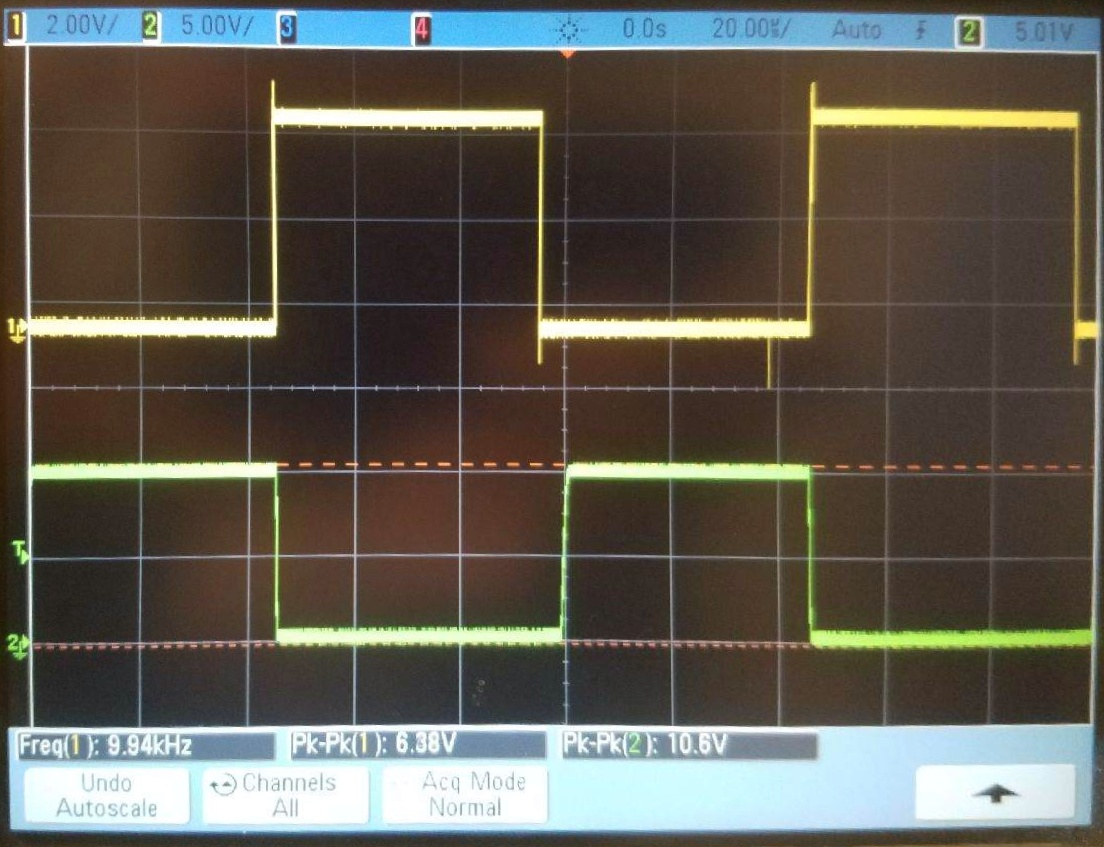
\includegraphics[scale=0.25]{../images/inverter_input_output.jpeg}
	\caption{Input and Output Signals of BJT Inverter}
	\label{fig:inverter_in_out}
\end{figure}
\FloatBarrier

{\footnotesize This image reflects the input and output of the same circuit in Figure \ref{fig:bjt_inverter}. However, the $V_{cc}$ value in this particular image is set to $10$\si{\volt} instead of $5$\si{\volt}. Because an image for $V_{cc} = 5$\si{\volt} was not taken, this image is used instead because the shape of the waveforms would be identical but with different amplitudes for the output signal.}

\FloatBarrier

When the square source is at its maximum, a large voltage is supplied to the base of the BJT. This translates to a forward-bias applied across the base-emitter junction and base-collector junction. At this point the BJT is operating in the saturation region. In the saturation region, the transistor effectively acts as a short circuit thus causing the output voltage at the emitter to be zero.

When the square source is at its minimum, essentially no voltage is supplied to the base of the BJT. As a result, the base-emitter junction and the base-collector junction are reverse biased and the BJT is operating in the cutoff region. In the cutoff region, the transistor effectively acts as an open circuit, so the output voltage at the emitter is equivalent to the value of $V_{cc}$.

By zooming in to the output signal, the rise and fall time of the signal can be measured.

\FloatBarrier
\begin{figure}[h!]
	\centering
	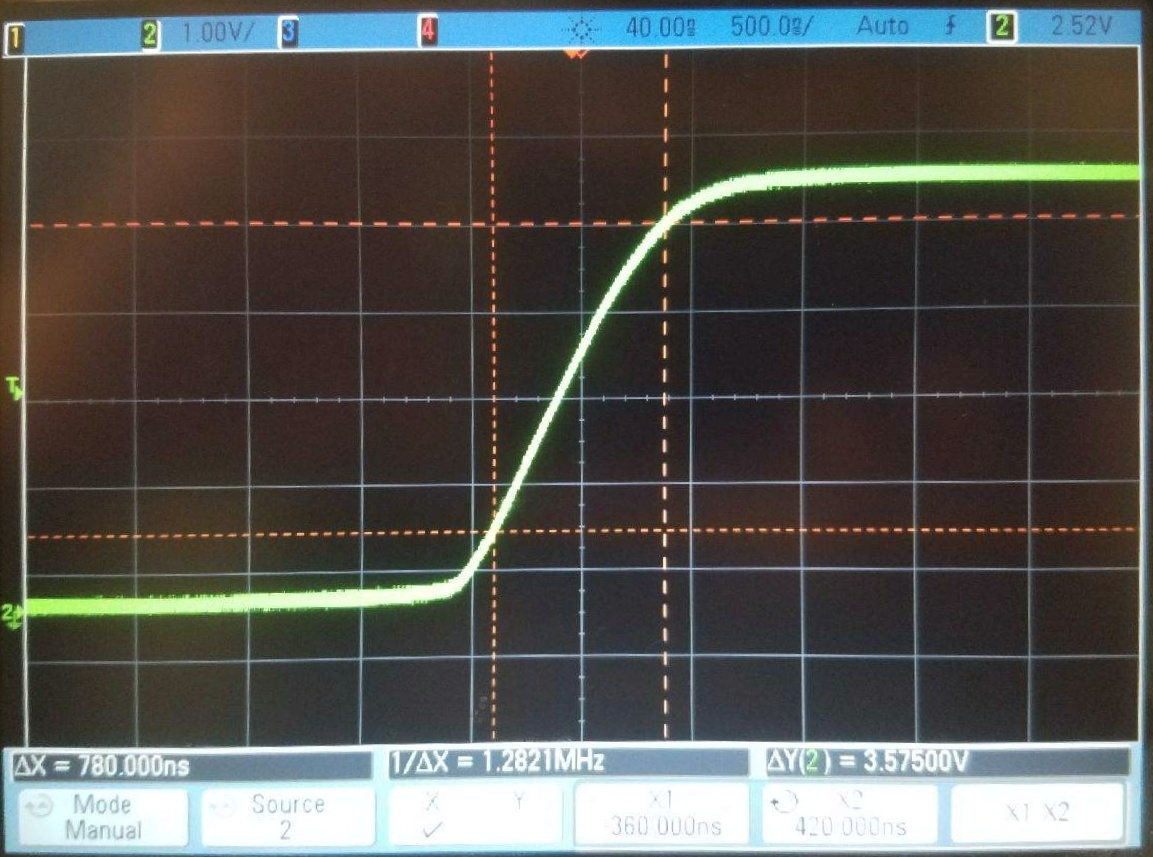
\includegraphics[scale=0.24]{../images/inverter_tr.jpeg}
	\caption{Rise Time of Output Signal}
	\label{fig:inverter_tr}
\end{figure}
\FloatBarrier

The rise time is found by measuring the difference in time of when the signal reaches $10\%$ of its relative maximum and when the signal reaches $90\%$ of its relative maximum at the rising edge. Using this method, the rise time of the output signal, $t_r$ is measured to be $780$\si{\nano\second}.

\FloatBarrier
\begin{figure}[h!]
	\centering
	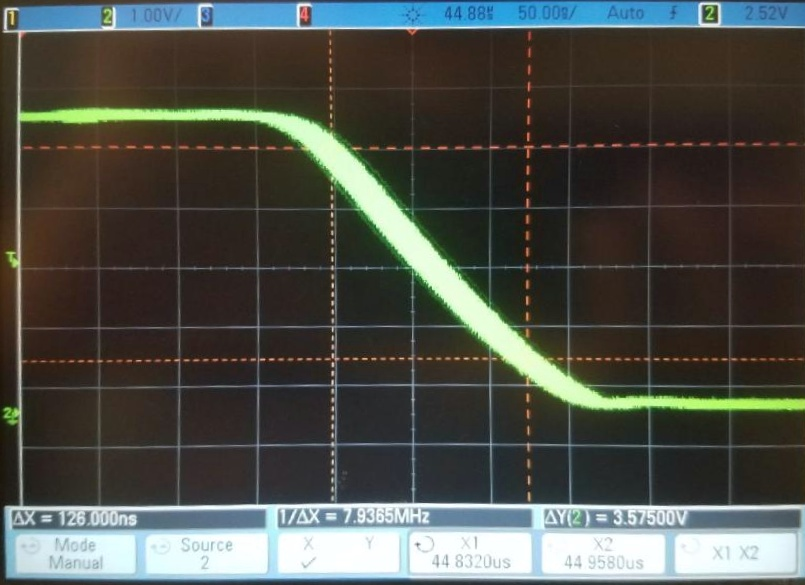
\includegraphics[scale=0.34]{../images/inverter_tf.jpeg}
	\caption{Fall Time of Output Signal}
	\label{fig:inverter_tf}
\end{figure}
\FloatBarrier

The fall time is found by measuring the difference between the time in which the signal reaches $90\%$ of its relative maximum and the time in which the signal reaches $10\%$ of its relative maximum at the falling edge. Using this method, the fall time of the output signal, $t_f$ is measured to be $126$\si{\nano\second}.

The delay times between the input and output signals for the saturation to cutoff transition and the cutoff to saturation transition of the BJT can be found by finding the difference between the time in which the input and output signals reach $50\%$ of their respective relative maxima. The measurement taken for the delay time for the saturation to cutoff transition of the BJT is shown in the following figure:

\FloatBarrier
\begin{figure}[h!]
	\centering
	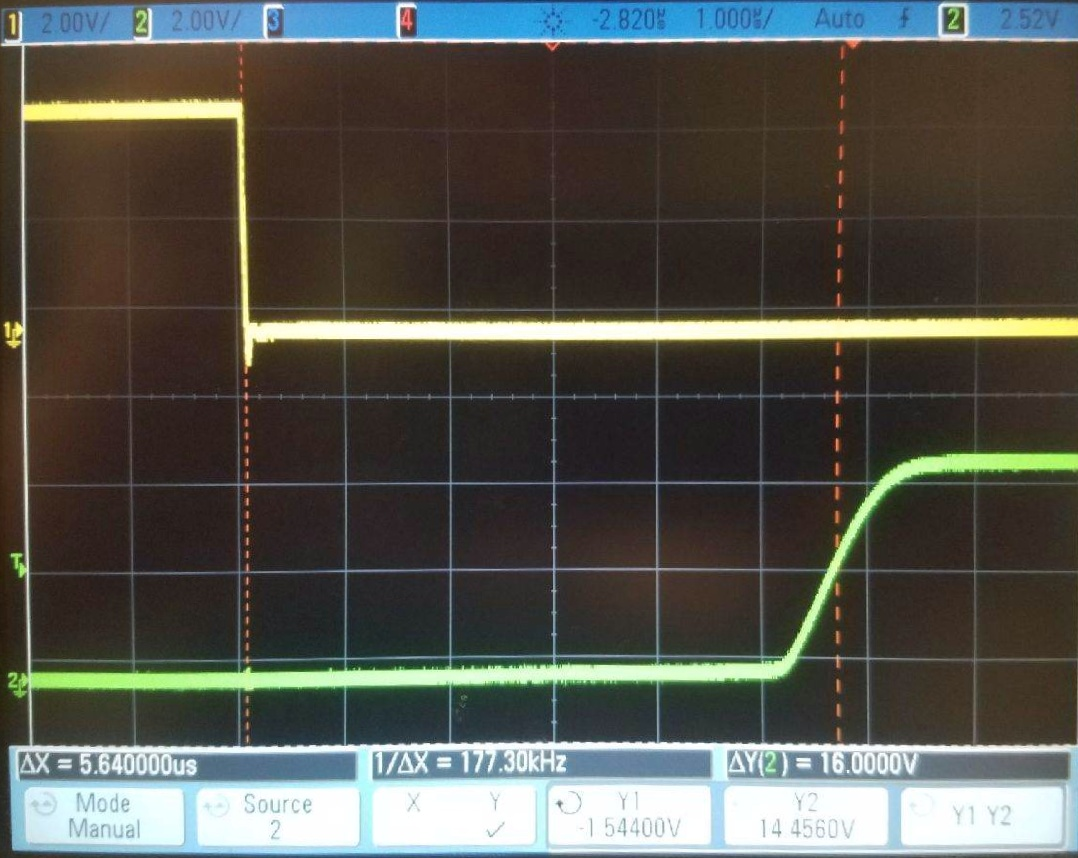
\includegraphics[scale=0.26]{../images/inverter_td.jpeg}
	\caption{Delay Time for Saturation to Cutoff Transition}
	\label{fig:inverter_td}
\end{figure}
\FloatBarrier

The delay time, $t_d$, for the saturation to cutoff transition of the BJT is measured to be $5.64$\si{\micro\second}. $t_d$ for the cutoff to saturation transition of the BJT is very close to the value found for $t_f$, and is approximately $130$\si{\nano\second}. The $t_d$ value for the saturation to cutoff transition is the more significant one by a large margin.

While the delay times are large for the BJT inverter circuit, they are still reasonable at $10$\si{\kilo\hertz}. This is because at $10$\si{\kilo\hertz}, the period of the wave is $0.1$\si{\milli\second}. The maxima and minima of a square wave at that frequency would then have a duration of $50$\si{\micro\second} which is significantly larger than the delay times, meaning their effects are relatively minimal. However, for high frequency applications, the BJT inverter circuit will fail. If the input signal has a frequency of $3$\si{\giga\hertz}, then the period of the wave would be $0.333$\si{\nano\second}. The delay times of the BJT inverter are orders of magnitudes larger than the period of the wave. Inversion of the input signal would not be observed because the slow switching time of the BJT.
\subsection{Amplifying Characteristics of the BJT}
\subsubsection{Gain and Frequency Response of Common-Emitter Amplifier}
This portion of the experiment demonstrates the amplification behavior of the inverter, also known as a common-emitter amplifier. Its properties are characterized by analyzing its gain and frequency response. \\
% Initial settings
The amplifier's input signal has a $200$\si{\milli\volt}pp amplitude and an $800$\si{\milli\volt}pp offset.
% At what point do distortions occur?
When the amplitude is increased to $400$\si{\milli\volt}pp, distortions occur in which the waveform becomes clipped. This is because the output waveform is amplified, but its peak and trough voltages are limited by the supply and ground voltages, respectively.
\FloatBarrier
\begin{figure}[h!]
	\centering
	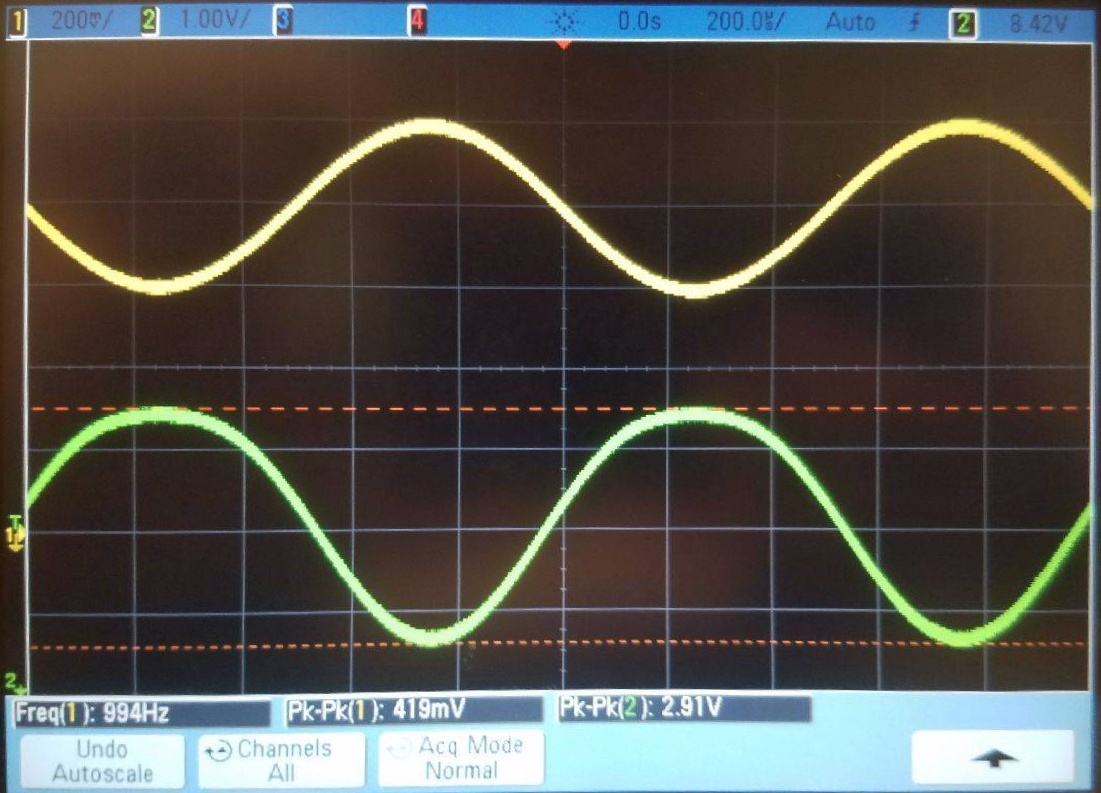
\includegraphics[scale=0.25]{./images/amplifier_10ghz_clamping.jpeg}
	\caption{Common-Emitter Amplifier $10$\si{\kilo\hertz} Distortions}
	\label{fig:clamping}
\end{figure}
\FloatBarrier
% Explanation of low-pass filtering with circuit diagram
The amplifier does not have a perfect frequency response due to the structure of the BJT used. The BJT has two pn-junctions, one between the collector and the base and one between the base and the emitter. Due to a variety of effects, the junctions each have an associated capacitance. At DC, current can easily flow through the BJT. Thus, these capacitances are not accurately modeled using a series capacitance since that would simply charge. A better model uses parallel capacitances, like in figure (\ref{fig:hf_bjt}) below:

\FloatBarrier
% NOTE: Circuit schematics MUST have labeled values.
\begin{figure}[h!]
	\centering
	\caption{High Frequency BJT Model}
	\label{fig:hf_bjt}
	\begin{circuitikz}
		\draw
		( 0 , 0 ) node[ npn ] (my_npn) {}

		% Base
		(my_npn.B) to [ short ] +( -3 , 0 ) coordinate(r_in)
		(r_in) to [ R={$10k\Omega$} ] ++( -3 , 0 ) coordinate(v_in)
		(v_in) to [ battery , v<=$V_{in}$ ] ++( 0 , -2 ) coordinate(gnd_1)
		(gnd_1) node[ ground ] (my_gnd_1) {}

		% Collector
		(my_npn.C) to [ short ] ++( 0 , 3 ) coordinate(r_c)
		(r_c) to [ R={$1k\Omega$} ] ++( 0 , 3 ) coordinate(vcc)
		(vcc) to [ battery , v<=$V_{cc}$ ] ++( 2 , 0 ) coordinate(gnd_3)
		(gnd_3) node[ ground ] (my_gnd_3) {}

		% Emitter
		(my_npn.E) to [ short ] ++( 0 , -3 ) coordinate(e_gnd)
		(e_gnd) node[ ground ] (my_e_gnd) {}

		% Parasitic Capacitances
		(r_c) to [ C ] (r_in)
		(my_e_gnd) to [ C ] (r_in)

		;
	\end{circuitikz}
\end{figure}

\FloatBarrier

At low frequencies, the parasitic capacitances acts as broken circuits. Thus, the circuit reduces to an ideal common-emitter amplifier. However, at higher frequencies, signals can short through the parasitic capacitances. Specifically, a short path exists between ground and the collector, making $V_{out} = 0$\si{\volt}. Thus, as frequency increases, the output voltage for a given input voltage, and therefore the gain, should drop. This is because gain is defined as $\frac{V_{out}}{V_{in}}$ [1].

% Gain at 10kHz
At $10$\si{\kilo\hertz}, the input voltage is the starting value of $200$\si{\milli\volt}pp, and the output voltage is 1.63\si{\volt}pp. Thus, the gain is $8.15$.
% How do you measure higher cutoff frequency?
Since parasitic capacitances should drop the gain at higher frequencies, a cutoff frequency can be defined. The cutoff frequency $f_c$ is the frequency at which the output voltage is $\frac{1}{\sqrt{2}}$ of the peak output voltage for a given input voltage [2]. So, in this case, $f_c$ is the frequency at which the output voltage is $\frac{1.63}{\sqrt{2}}$ \si{\volt}pp $ \approx 1.15$ \si{\volt}pp. This can be measured by simply increasing the frequency until an output voltage amplitude of $1.15$ \si{\volt}pp occurs.
% What was our measured cutoff frequency?
Using this method, the cutoff frequency $f_c \approx 150$\si{\kilo\hertz} is obtained.
% Gain at cutoff frequency
At this point, the gain is approximately $5.75$.
% Table with gains at different frequencies
\FloatBarrier
\begin{table}[h!]
	\centering
	\caption{Common-Emitter Amplifier Frequency Response}
	\label{tab:cea_response}
	\csvautotabular{./tables/amplifier_gains.csv}
\end{table}
\FloatBarrier
\subsubsection{Square Wave Response of Common-Emitter Amplifier}
% Output signal vs square wave input
The frequency of the square wave response is set to the cutoff frequency $f_c = 150$\si{\kilo\hertz}. In order to understand the square wave response of a common-emitter amplifier, the 20\% duty cycle case is considered first. Clearly, the output waveform differs considerably from the input waveform, unlike the earlier inverter experiment. This is because of delays in the BJT's response.
\FloatBarrier
\begin{figure}[h!]
	\centering
	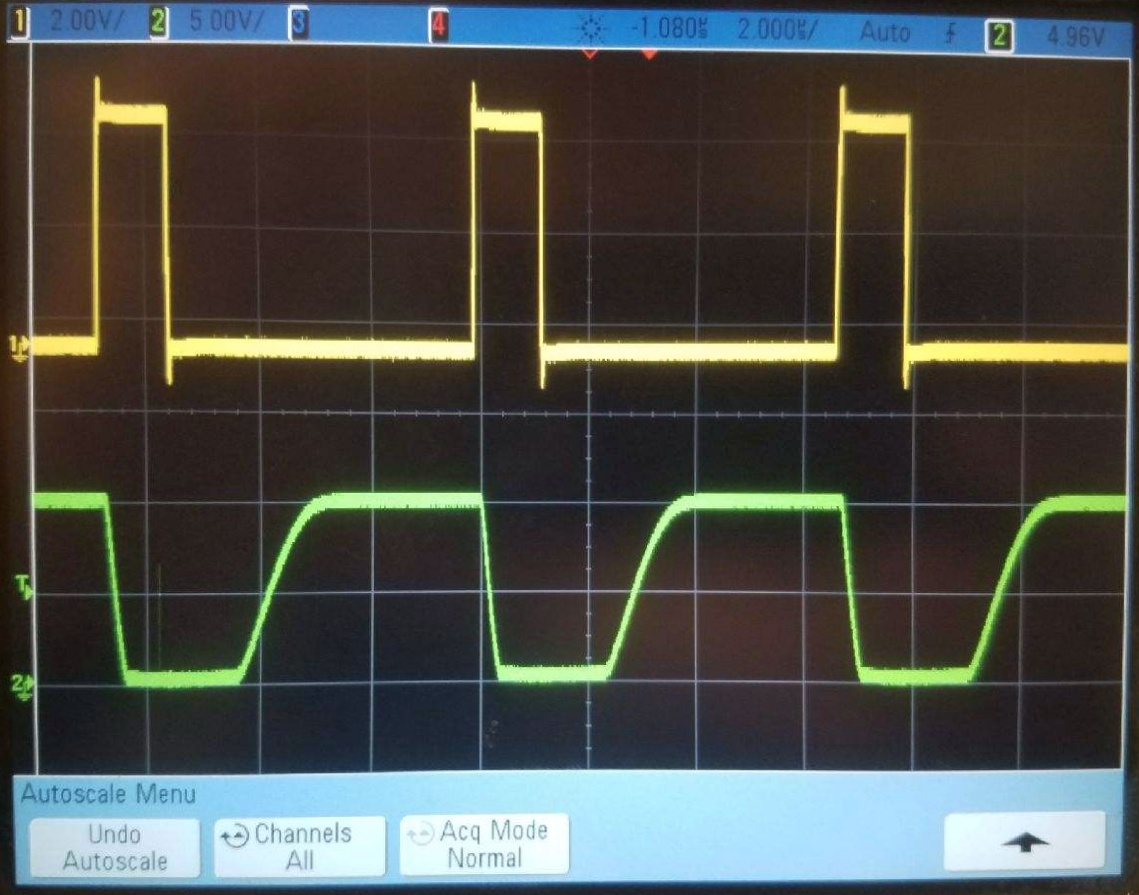
\includegraphics[scale=0.25]{./images/amplifier_20_duty_cycle.jpeg}
	\caption{Common-Emitter Amplifier Square Wave Response 20\% Duty Cycle}
	\label{fig:twenty_perc_duty_cycle}
\end{figure}
\FloatBarrier
When the square wave pulse is high, the output drops nearly to ground due to the inverting characteristics of the amplifier. When the input drops to ground, the output gradually becomes high for the same reason. There is a brief delay between the falling edge of the input waveform and the rising "edge" of the output waveform. This is because the capacitors in figure (\ref{fig:hf_bjt}) need to charge first before the low-pass filter's DC characteristics take over. The charging and discharging of the capacitors represents the formation and destruction of the depletion regions in the BJT. \\
The reason the output waveform appears to saturate is because the duty cycle is low enough that the input signal remains low for long enough that a steady state can be established. It saturates at $10$\si{\volt}, the supply voltage, because the output voltage cannot exceed supply. The amplifier operates on the principle of using the weaker signal to enable or disable a transistor switch that controls a larger voltage. This larger voltage is the supply voltage, which is why the output cannot exceed supply. \\
When the duty cycle is increased to 50\%, the same physical principles still apply.
\FloatBarrier
\begin{figure}[h!]
	\centering
	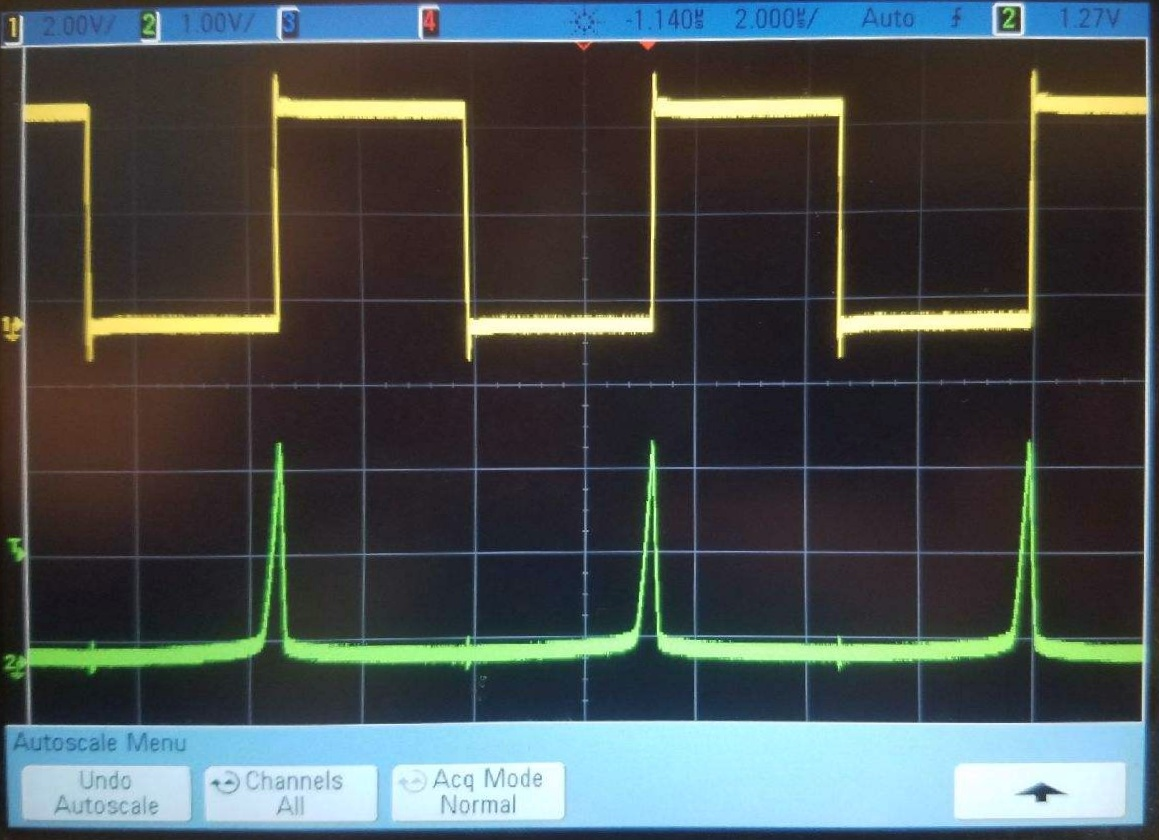
\includegraphics[scale=0.25]{./images/amplifier_50_duty_cycle.jpeg}
	\caption{Common-Emitter Amplifier Square Wave Response 50\% Duty Cycle}
	\label{fig:fifty_perc_duty_cycle}
\end{figure}
\FloatBarrier
The output waveform waits for a time delay and then begins to develop. However, because the duty cycle is longer, the input signal remains low for a shorter period of time. Thus, the output voltage does not have a sufficient amount of time to fully develop and is cut short when the rising edge of the input occurs. \\
% Why is there distortion
% TODO Add values to circuit schematics. TODO Discussion. TODO Tell Jason to put values in circuit schematics and explain why inverting amplifier works. Send him your prelab which explains why.

\section{Discussion}
\subsection{Inverting Characteristics of the BJT}
\subsubsection{Output Signal of Inverter Circuit}

The inverter circuit is constructed using a BJT. The input and output signals of the BJT inverter circuit are analyzed to determine its unique properties. The output signal is taken from the collector of the BJT in the circuit, which can be visualized below:

\FloatBarrier
\begin{figure}[h!]
	\centering
	\caption{BJT Inverter Circuit}
	\label{fig:bjt_inverter}
	\begin{circuitikz}
		\draw
		( 0 , 0 ) node[ npn ] (my_npn) {$V_{out}$}
		
		% Base
		(my_npn.B) to [ short ] +( -2 , 0 ) coordinate(r_in)
		(r_in) to [ R={$10k\Omega$} ] ++( -2 , 0 ) coordinate(v_in)
		(v_in) to [ sqV , v<=$V_{in}$ ] ++( 0 , -2 ) coordinate(gnd_1)
		(gnd_1) node[ ground ] (my_gnd_1) {}
		
		% Collector
		(my_npn.C) to [ short ] ++( 0 , 2 ) coordinate(r_c)
		(r_c) to [ R={$1k\Omega$} ] ++( 0 , 2 ) coordinate(vcc)
		(vcc) to [ battery , v<=$V_{cc}$ ] ++( 2 , 0 ) coordinate(gnd_3)
		(gnd_3) node[ ground ] (my_gnd_3) {}
		
		% Emitter
		(my_npn.E) to [ short ] ++( 0 , -2 ) coordinate(e_gnd)
		(e_gnd) node[ ground ] (my_e_gnd) {}
		
		;
	\end{circuitikz}
\end{figure}

\FloatBarrier

By supplying the inverter with a $10$\si{\kilo\hertz} square input signal with fixed minimum and maximum values at $0$\si{\volt} and $5$\si{\volt} respectively with a $50\%$ duty cycle and a $V_{cc}$ value of $5$\si{\volt}, the following input and output signals are observed on the oscilloscope:

\FloatBarrier
\begin{figure}[h!]
	\centering
	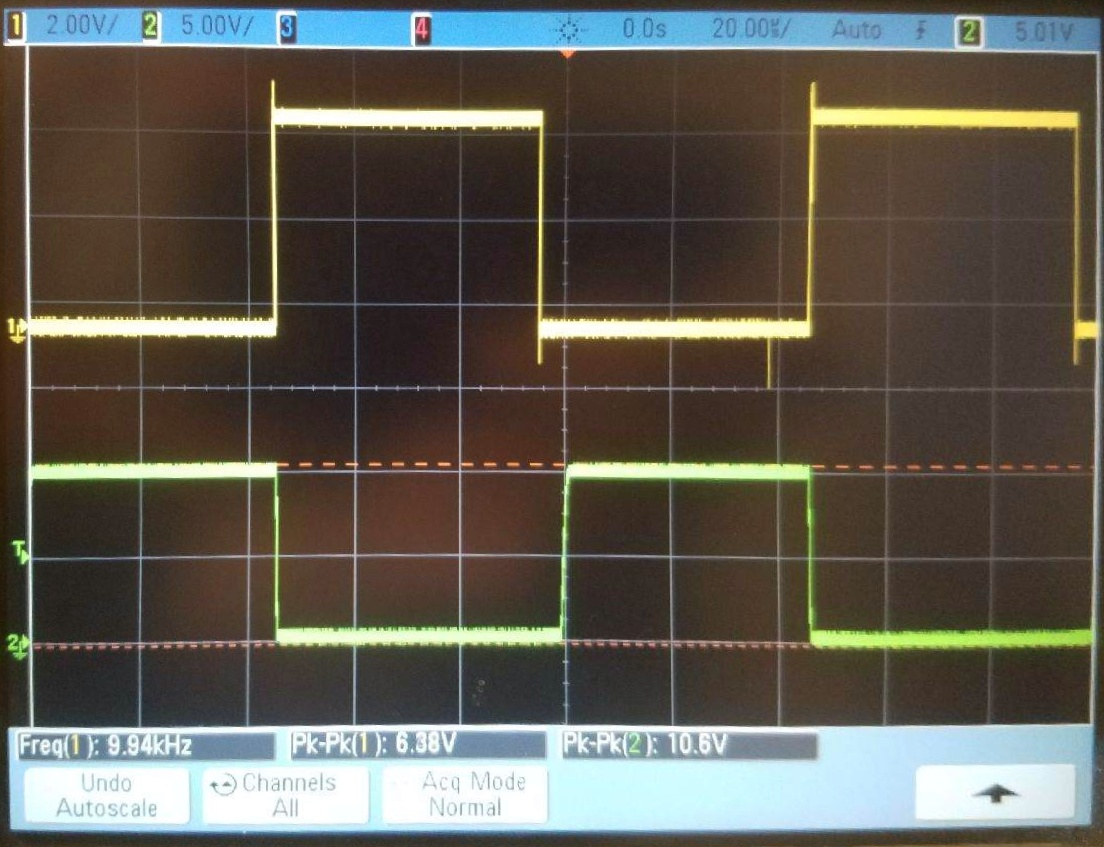
\includegraphics[scale=0.25]{../images/inverter_input_output.jpeg}
	\caption{Input and Output Signals of BJT Inverter}
	\label{fig:inverter_in_out}
\end{figure}
\FloatBarrier

{\footnotesize This image reflects the input and output of the same circuit in Figure \ref{fig:bjt_inverter}. However, the $V_{cc}$ value in this particular image is set to $10$\si{\volt} instead of $5$\si{\volt}. Because an image for $V_{cc} = 5$\si{\volt} was not taken, this image is used instead because the shape of the waveforms would be identical but with different amplitudes for the output signal.}

\FloatBarrier

When the square source is at its maximum, a large voltage is supplied to the base of the BJT. This translates to a forward-bias applied across the base-emitter junction and base-collector junction. At this point the BJT is operating in the saturation region. In the saturation region, the transistor effectively acts as a short circuit thus causing the output voltage at the emitter to be zero.

When the square source is at its minimum, essentially no voltage is supplied to the base of the BJT. As a result, the base-emitter junction and the base-collector junction are reverse biased and the BJT is operating in the cutoff region. In the cutoff region, the transistor effectively acts as an open circuit, so the output voltage at the emitter is equivalent to the value of $V_{cc}$.

By zooming in to the output signal, the rise and fall time of the signal can be measured.

\FloatBarrier
\begin{figure}[h!]
	\centering
	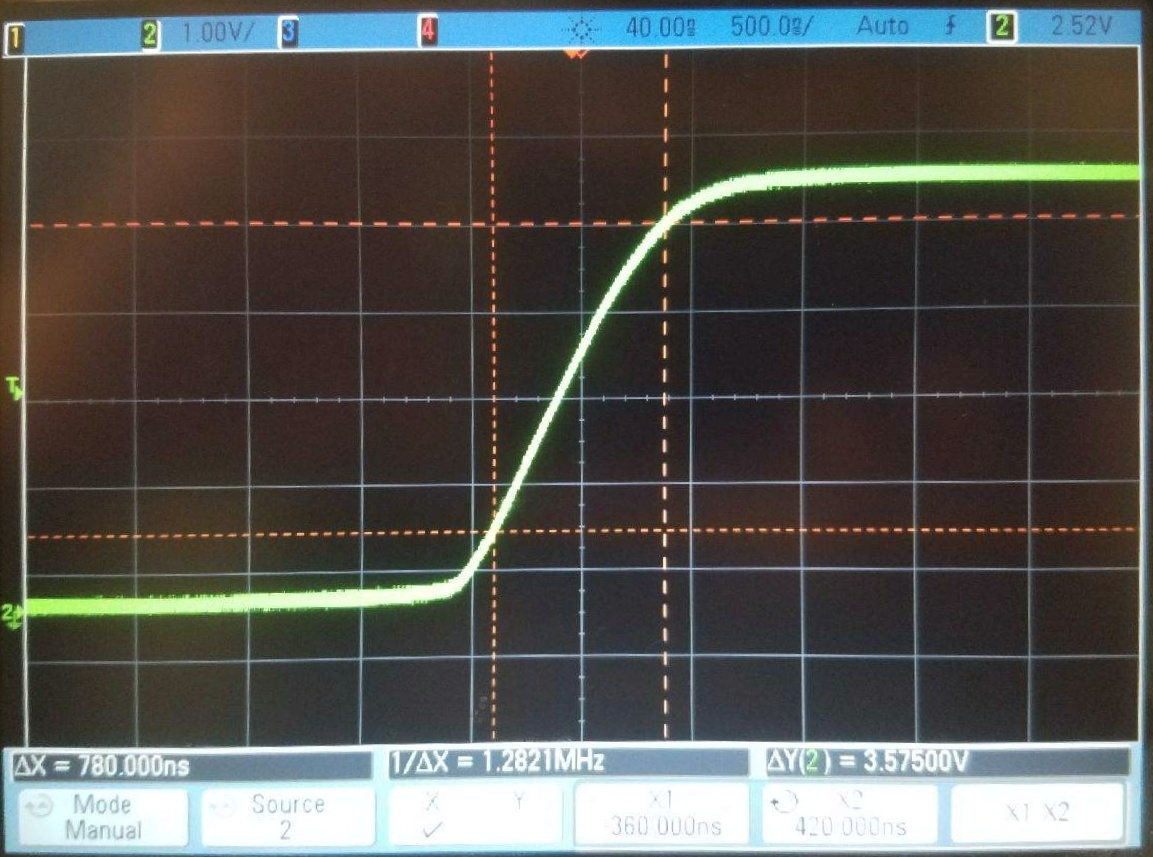
\includegraphics[scale=0.24]{../images/inverter_tr.jpeg}
	\caption{Rise Time of Output Signal}
	\label{fig:inverter_tr}
\end{figure}
\FloatBarrier

The rise time is found by measuring the difference in time of when the signal reaches $10\%$ of its relative maximum and when the signal reaches $90\%$ of its relative maximum at the rising edge. Using this method, the rise time of the output signal, $t_r$ is measured to be $780$\si{\nano\second}.

\FloatBarrier
\begin{figure}[h!]
	\centering
	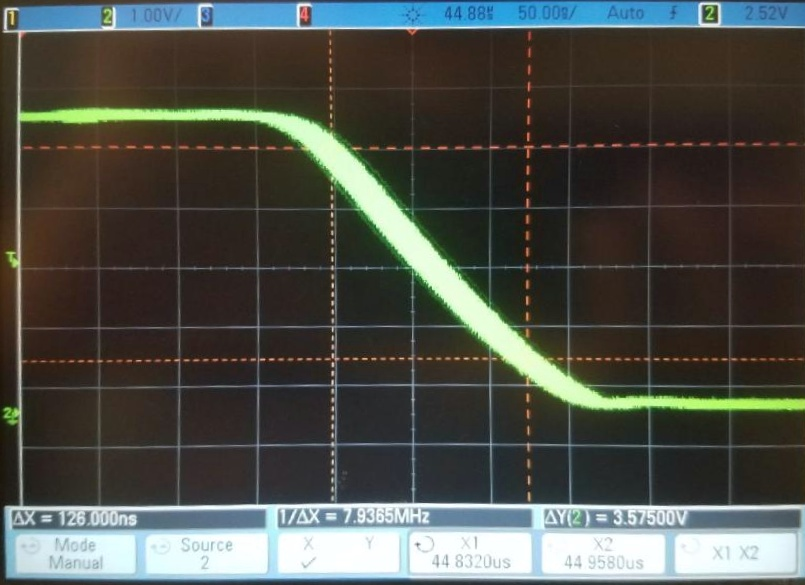
\includegraphics[scale=0.34]{../images/inverter_tf.jpeg}
	\caption{Fall Time of Output Signal}
	\label{fig:inverter_tf}
\end{figure}
\FloatBarrier

The fall time is found by measuring the difference between the time in which the signal reaches $90\%$ of its relative maximum and the time in which the signal reaches $10\%$ of its relative maximum at the falling edge. Using this method, the fall time of the output signal, $t_f$ is measured to be $126$\si{\nano\second}.

The delay times between the input and output signals for the saturation to cutoff transition and the cutoff to saturation transition of the BJT can be found by finding the difference between the time in which the input and output signals reach $50\%$ of their respective relative maxima. The measurement taken for the delay time for the saturation to cutoff transition of the BJT is shown in the following figure:

\FloatBarrier
\begin{figure}[h!]
	\centering
	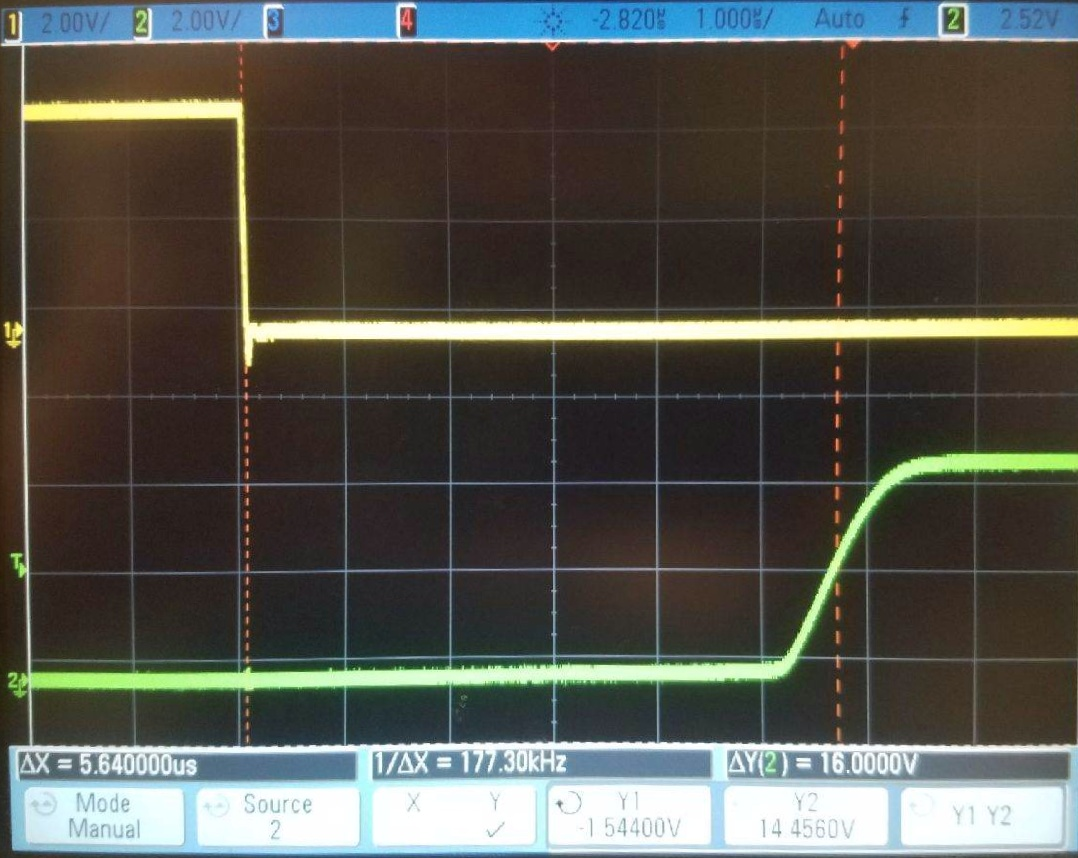
\includegraphics[scale=0.26]{../images/inverter_td.jpeg}
	\caption{Delay Time for Saturation to Cutoff Transition}
	\label{fig:inverter_td}
\end{figure}
\FloatBarrier

The delay time, $t_d$, for the saturation to cutoff transition of the BJT is measured to be $5.64$\si{\micro\second}. $t_d$ for the cutoff to saturation transition of the BJT is very close to the value found for $t_f$, and is approximately $130$\si{\nano\second}. The $t_d$ value for the saturation to cutoff transition is the more significant one by a large margin.

While the delay times are large for the BJT inverter circuit, they are still reasonable at $10$\si{\kilo\hertz}. This is because at $10$\si{\kilo\hertz}, the period of the wave is $0.1$\si{\milli\second}. The maxima and minima of a square wave at that frequency would then have a duration of $50$\si{\micro\second} which is significantly larger than the delay times, meaning their effects are relatively minimal. However, for high frequency applications, the BJT inverter circuit will fail. If the input signal has a frequency of $3$\si{\giga\hertz}, then the period of the wave would be $0.333$\si{\nano\second}. The delay times of the BJT inverter are orders of magnitudes larger than the period of the wave. Inversion of the input signal would not be observed because the slow switching time of the BJT.
\subsection{Amplifying Characteristics of the BJT}
\subsubsection{Gain and Frequency Response of Common-Emitter Amplifier}
This portion of the experiment demonstrates the amplification behavior of the inverter, also known as a common-emitter amplifier. Its properties are characterized by analyzing its gain and frequency response. \\
% Initial settings
The amplifier's input signal has a $200$\si{\milli\volt}pp amplitude and an $800$\si{\milli\volt}pp offset.
% At what point do distortions occur?
When the amplitude is increased to $400$\si{\milli\volt}pp, distortions occur in which the waveform becomes clipped. This is because the output waveform is amplified, but its peak and trough voltages are limited by the supply and ground voltages, respectively.
\FloatBarrier
\begin{figure}[h!]
	\centering
	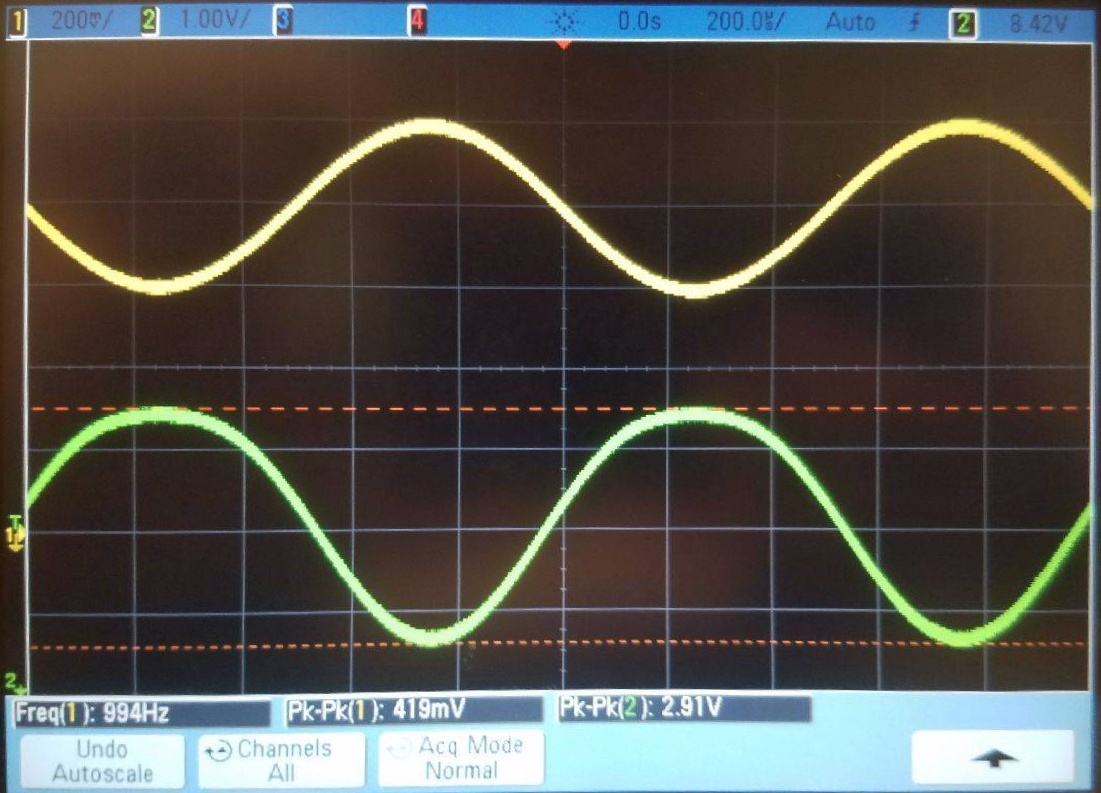
\includegraphics[scale=0.25]{./images/amplifier_10ghz_clamping.jpeg}
	\caption{Common-Emitter Amplifier $10$\si{\kilo\hertz} Distortions}
	\label{fig:clamping}
\end{figure}
\FloatBarrier
% Explanation of low-pass filtering with circuit diagram
The amplifier does not have a perfect frequency response due to the structure of the BJT used. The BJT has two pn-junctions, one between the collector and the base and one between the base and the emitter. Due to a variety of effects, the junctions each have an associated capacitance. At DC, current can easily flow through the BJT. Thus, these capacitances are not accurately modeled using a series capacitance since that would simply charge. A better model uses parallel capacitances, like in figure (\ref{fig:hf_bjt}) below:

\FloatBarrier
% NOTE: Circuit schematics MUST have labeled values.
\begin{figure}[h!]
	\centering
	\caption{High Frequency BJT Model}
	\label{fig:hf_bjt}
	\begin{circuitikz}
		\draw
		( 0 , 0 ) node[ npn ] (my_npn) {}

		% Base
		(my_npn.B) to [ short ] +( -3 , 0 ) coordinate(r_in)
		(r_in) to [ R={$10k\Omega$} ] ++( -3 , 0 ) coordinate(v_in)
		(v_in) to [ battery , v<=$V_{in}$ ] ++( 0 , -2 ) coordinate(gnd_1)
		(gnd_1) node[ ground ] (my_gnd_1) {}

		% Collector
		(my_npn.C) to [ short ] ++( 0 , 3 ) coordinate(r_c)
		(r_c) to [ R={$1k\Omega$} ] ++( 0 , 3 ) coordinate(vcc)
		(vcc) to [ battery , v<=$V_{cc}$ ] ++( 2 , 0 ) coordinate(gnd_3)
		(gnd_3) node[ ground ] (my_gnd_3) {}

		% Emitter
		(my_npn.E) to [ short ] ++( 0 , -3 ) coordinate(e_gnd)
		(e_gnd) node[ ground ] (my_e_gnd) {}

		% Parasitic Capacitances
		(r_c) to [ C ] (r_in)
		(my_e_gnd) to [ C ] (r_in)

		;
	\end{circuitikz}
\end{figure}

\FloatBarrier

At low frequencies, the parasitic capacitances acts as broken circuits. Thus, the circuit reduces to an ideal common-emitter amplifier. However, at higher frequencies, signals can short through the parasitic capacitances. Specifically, a short path exists between ground and the collector, making $V_{out} = 0$\si{\volt}. Thus, as frequency increases, the output voltage for a given input voltage, and therefore the gain, should drop. This is because gain is defined as $\frac{V_{out}}{V_{in}}$ [1].

% Gain at 10kHz
At $10$\si{\kilo\hertz}, the input voltage is the starting value of $200$\si{\milli\volt}pp, and the output voltage is 1.63\si{\volt}pp. Thus, the gain is $8.15$.
% How do you measure higher cutoff frequency?
Since parasitic capacitances should drop the gain at higher frequencies, a cutoff frequency can be defined. The cutoff frequency $f_c$ is the frequency at which the output voltage is $\frac{1}{\sqrt{2}}$ of the peak output voltage for a given input voltage [2]. So, in this case, $f_c$ is the frequency at which the output voltage is $\frac{1.63}{\sqrt{2}}$ \si{\volt}pp $ \approx 1.15$ \si{\volt}pp. This can be measured by simply increasing the frequency until an output voltage amplitude of $1.15$ \si{\volt}pp occurs.
% What was our measured cutoff frequency?
Using this method, the cutoff frequency $f_c \approx 150$\si{\kilo\hertz} is obtained.
% Gain at cutoff frequency
At this point, the gain is approximately $5.75$.
% Table with gains at different frequencies
\FloatBarrier
\begin{table}[h!]
	\centering
	\caption{Common-Emitter Amplifier Frequency Response}
	\label{tab:cea_response}
	\csvautotabular{./tables/amplifier_gains.csv}
\end{table}
\FloatBarrier
\subsubsection{Square Wave Response of Common-Emitter Amplifier}
% Output signal vs square wave input
The frequency of the square wave response is set to the cutoff frequency $f_c = 150$\si{\kilo\hertz}. In order to understand the square wave response of a common-emitter amplifier, the 20\% duty cycle case is considered first. Clearly, the output waveform differs considerably from the input waveform, unlike the earlier inverter experiment. This is because of delays in the BJT's response.
\FloatBarrier
\begin{figure}[h!]
	\centering
	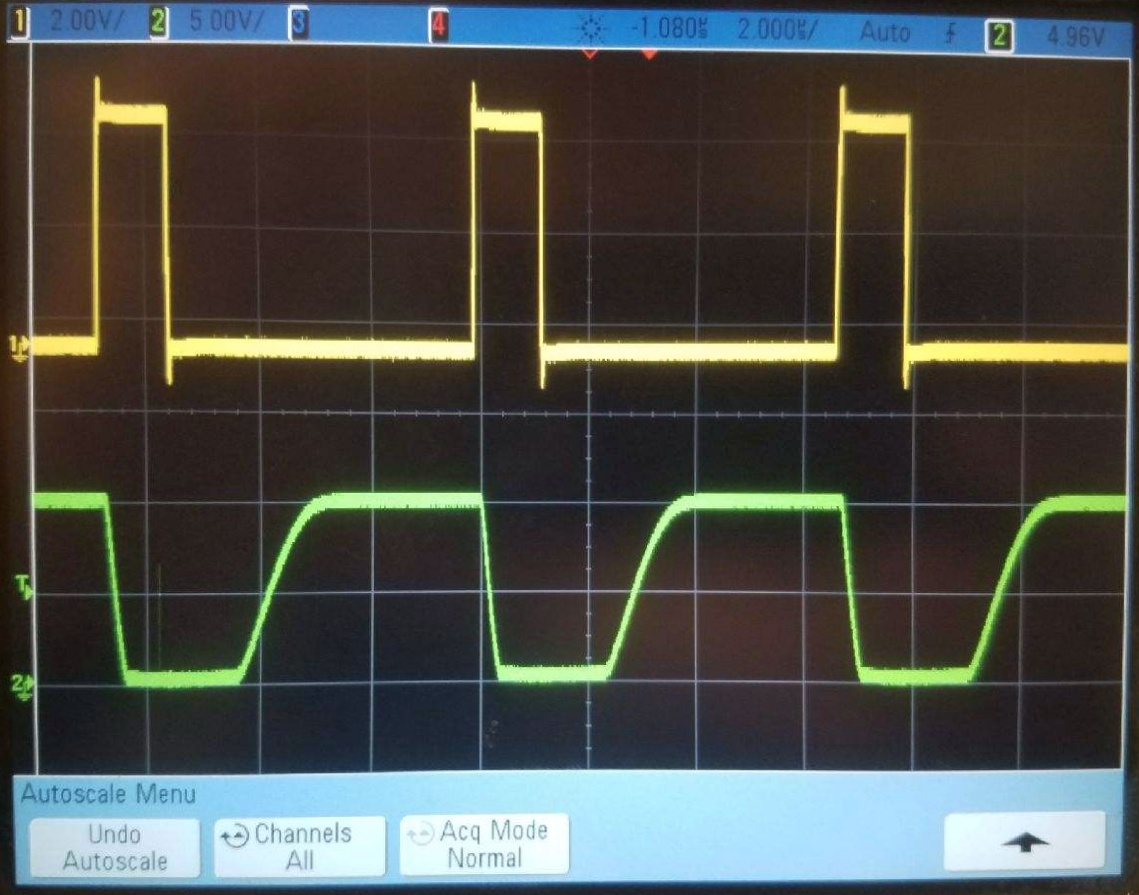
\includegraphics[scale=0.25]{./images/amplifier_20_duty_cycle.jpeg}
	\caption{Common-Emitter Amplifier Square Wave Response 20\% Duty Cycle}
	\label{fig:twenty_perc_duty_cycle}
\end{figure}
\FloatBarrier
When the square wave pulse is high, the output drops nearly to ground due to the inverting characteristics of the amplifier. When the input drops to ground, the output gradually becomes high for the same reason. There is a brief delay between the falling edge of the input waveform and the rising "edge" of the output waveform. This is because the capacitors in figure (\ref{fig:hf_bjt}) need to charge first before the low-pass filter's DC characteristics take over. The charging and discharging of the capacitors represents the formation and destruction of the depletion regions in the BJT. \\
The reason the output waveform appears to saturate is because the duty cycle is low enough that the input signal remains low for long enough that a steady state can be established. It saturates at $10$\si{\volt}, the supply voltage, because the output voltage cannot exceed supply. The amplifier operates on the principle of using the weaker signal to enable or disable a transistor switch that controls a larger voltage. This larger voltage is the supply voltage, which is why the output cannot exceed supply. \\
When the duty cycle is increased to 50\%, the same physical principles still apply.
\FloatBarrier
\begin{figure}[h!]
	\centering
	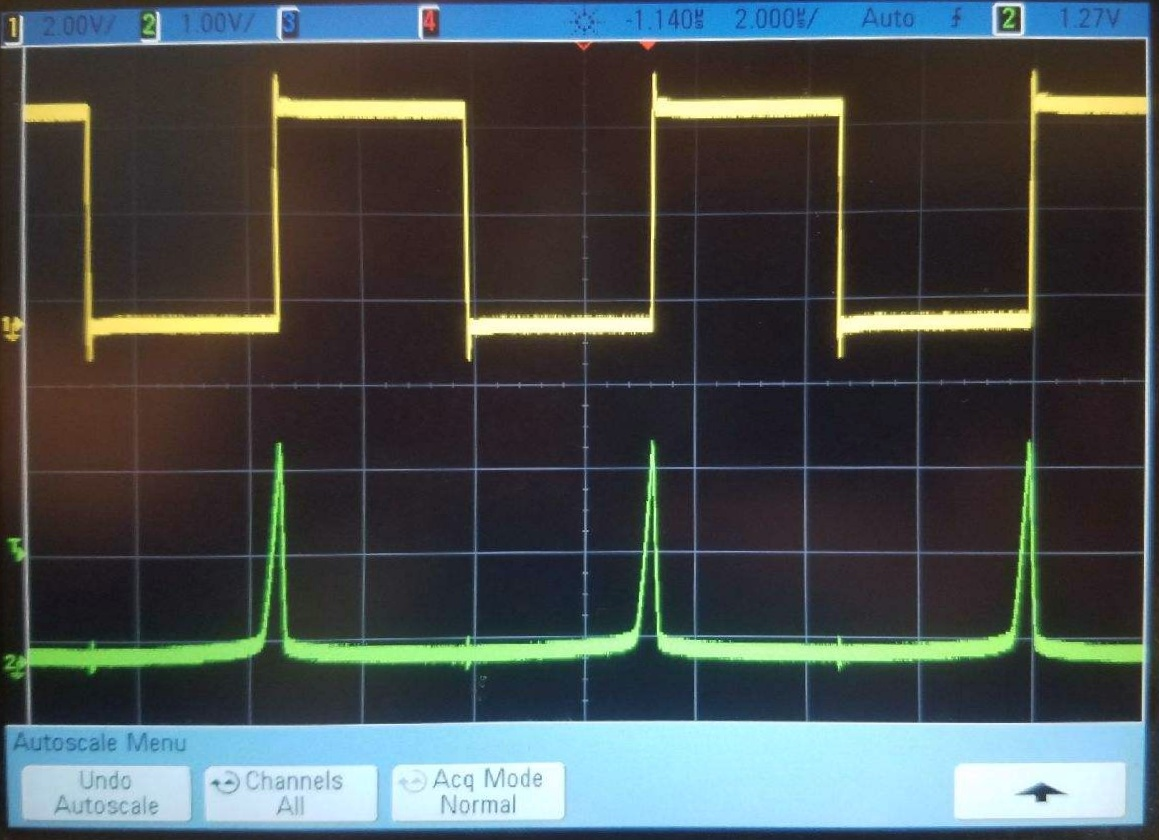
\includegraphics[scale=0.25]{./images/amplifier_50_duty_cycle.jpeg}
	\caption{Common-Emitter Amplifier Square Wave Response 50\% Duty Cycle}
	\label{fig:fifty_perc_duty_cycle}
\end{figure}
\FloatBarrier
The output waveform waits for a time delay and then begins to develop. However, because the duty cycle is longer, the input signal remains low for a shorter period of time. Thus, the output voltage does not have a sufficient amount of time to fully develop and is cut short when the rising edge of the input occurs. \\
% Why is there distortion
% TODO Add values to circuit schematics. TODO Discussion. TODO Tell Jason to put values in circuit schematics and explain why inverting amplifier works. Send him your prelab which explains why.

\section{References}
1. \url{http://www.ittc.ku.edu/~jstiles/412/handouts/5.8\%20BJT\%20Internal\%20Capacitances\%20and\%20high\%20frequency\%20model/section\%205_8\%20BJT\%20Internal\%20Capacitances\%20lecture.pdf} \\ %ref:bjt_cap
2. \url{http://alignment.hep.brandeis.edu/Lab/Filter/Filter.html} \\ %ref:cutoff_freq
\end{document}
